%___________________________________________
%*************************************************************
% Learning
%___________________________________________
%^^^^^^^^^^^^^^^^^^^^^^^^^^^^^^^^^^^^^^^^^^^^^^^^^^^

\section{Learning}

The learning module's goal is to utilise the ECJ library to evolve a population of byte vectors (representing agent rulesets). This is achieved through extending ECJ's classes, in conjunction with a parameter file. The ECJ library is an extensive collection of learning processes and, due to the limitations of this report, only the relevant sections, and the extensions thereof, are described. An important part of the project was adjusting the parameter file in reaction to previous learning runs, these revisions are discussed in Section \ref{subsec:learnparam}. However, some parameters were deemed fundamental and stayed invariant throughout this process; these are described, alongside the general evolutionary approach, in the following section.

%-----------------------------------------------------------------------
% Design
%-----------------------------------------------------------------------

\subsection{Evolutionary Approach}
\label{subsec:learndes}

Similar to the approach taken in developing the REALM agent (described in Section \ref{ssec:realm}), this project uses a  $(\mu  + \lambda)$ evolution strategy. However, unlike REALM, it focuses purely on mutation, with no crossover between individuals (a technique not traditionally applied with ESes \cite[p.~]{ecj-tut3}).

Evolution runs for 1000 generations with a population size of 50. The truncation selection size for our ES ($\mu$) is set to 5. Hence, the top 5 fittest individuals are chosen each generation. These are cloned and mutated to form 45 ($\lambda$) new individuals, which are then joined by the original 5 for the next generation.

Each individual's genome is a byte vector of length 300, representing a ruleset containing 20 rules. The default action is fixed over all rulesets and is specified by the parameter file.

Each element of the genome (a gene) has several mutation parameters associated to it. During the mutation phase each gene will be mutated with the probability prescribed by its mutation probability. Each gene can be mutating in one of two ways. The first will simply choose a random byte between its minimum and maximum values (inclusive), known as \textbf{reset} mutation. The second will favour one particular byte value, with a certain probability, which is known as \textbf{favour} mutation. Which method of mutation a gene undergoes, as well as the favoured byte and its probability are all contained in the individual gene's parameters, allowing for very fine grained control over the mutation process.

The evaluation stage takes each individual's genome and constructs an agent. The individual's fitness is calculated by passing the agent to the MWEvaluationTask, which has been initialised with a fixed set of level playing parameters decreed by the parameter file. These parameters have a custom set of evaluation multipliers and describe a task of 10 levels, varying level options for each level. Each generation builds this task with its own unique level seed to avoid over-fitting to one set of generated levels.

Statistics for average and best fitness are logged each generation. Level seed is also reported, to allow direct comparison between the learning process and the hand-crafted agents. After the final generation a selection of agents are written to agent files, including the best individual of the final generation and the best individual over all generations.

%-----------------------------------------------------------------------
% Extending the ECJ Library
%-----------------------------------------------------------------------

\subsection{The ECJ Library}

\begin{figure}[t]
	\centering
	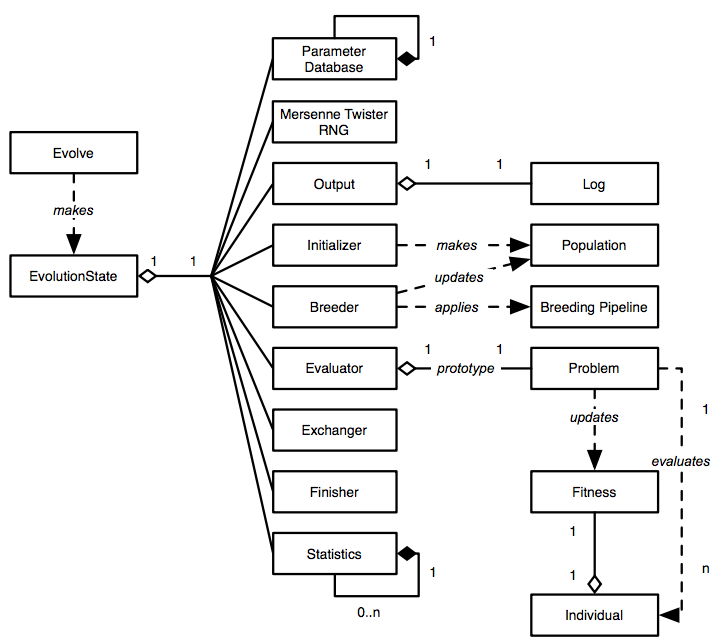
\includegraphics[scale=0.5]{ECJTopLevel.png}
	\caption{A top-level UML class diagram of the operation facilities in EvolutionState, taken from \cite[p.~10]{ecj-manual}.}
	\label{fig:ecjop}
\end{figure}

\begin{figure}[t]
	\centering
	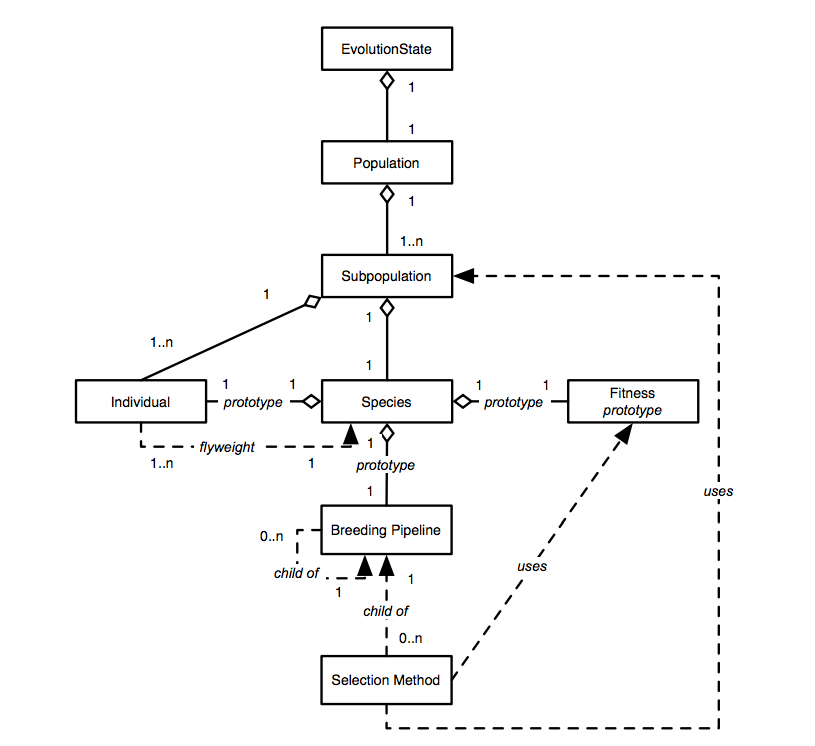
\includegraphics[scale=0.5]{ECJTopLevelData.png}
	\caption{A top-level UML class diagram of ECJ's data objects, taken from \cite[p.~11]{ecj-manual}.}
	\label{fig:ecjdata}
\end{figure}

\begin{figure}[t]
	\centering
	\includegraphics[scale=0.5]{LearningClassDiagram.png}
	\caption{A simplified UML class diagram of the Learning module's extension to ECJ.}
	\label{fig:lucl}
\end{figure}


The primary method for specialising ECJ for a particular use case is to extend the classes it provides, and specify these subclasses, alongside other pertinent values, in the parameter file. Nearly every method in ECJ's classes is passed the pseudo-global EvolutionState singleton, which holds instances of all other classes in use. A top-level view of ECJ's structure can be found in Figures \ref{fig:ecjop} and \ref{fig:ecjdata}.

The learning module will be built on top of the ECJ library, with a view to adhering to its style and ideology. For our approach, several of ECJ's classes did not need to extended, and simply specifying their default implementations in the parameter file was enough. The classes of interest to this project are the following: \emph{Species}, \emph{Individual}, \emph{SelectionMethod}, \emph{Breeder}, \emph{BreedingPipeline}, \emph{Evaluator}, \emph{Problem} and \emph{Statisitics}. A simplified class diagram of the learning module is included as Figure \ref{fig:lucl}.

ECJ provides the \emph{ByteVectorIndividual} class, which contains a Java array of \emph{byte}s, this is used to hold individual byte vector genomes. It also decrees the use of the \emph{IntegerVectorSpecies} class, which holds the gene parameters (e.g. minimum value, mutation probability). Our design first extends this class to the \emph{DynamicParameterIntegerVectorSpecies} class, which holds a subclass instance of another new class, the \emph{DynamicSpeciesParameters} class. The specific subclass to be used is specified in the parameter file. The purpose of this class is to provide a facility to override the min, max and mutation probability properties of each gene directly from the agent framework (rather than the parameter file). This class is then further extended to the \emph{RulesetSpecies} class, which holds gene parameters pertaining to favour mutation. This class also extends the parameter file's vocabulary to allow gene parameters to specified on a \textbf{condition} or \textbf{action} (the composite parts of a rule) basis. For example, the favour byte for all genes that represent conditions can be set as follows in the parameter file:

\begin{minipage}{0.9\linewidth}
\centering
\begin{lstlisting}
   ...species.condition.favour_byte 	= -1
\end{lstlisting}
\end{minipage}


The \emph{SelectionMethod} and \emph{Breeder} classes are responsible for selecting individuals (based on fitness) to clone and pass to the breeding pipeline. ECJ natively supports evolution strategies and so it is enough to specify these classes to be ECJ's \emph{ESSelection} and \emph{MuPlusLambda} classes. The \emph{BreedingPipeline} extension, \emph{RulesetMutationPipeline}, performs the mutation of individuals. For each gene in a individual's genome it requests the corresponding mutation parameters from the species class. It then clones and, if required, mutates the gene with either favour or reset mutation. 

The \emph{Evaluator} class is responsible for threading and batching the individuals to have their fitness calculated by cloned instances of the \emph{Problem} class. Hence, only the Problem class is extended, to the \emph{AgentRulesetEvaluator} class. On initialisation this class reads the the level options from the parameter file using the EvaluationParamsUtil class described in Section \ref{subsec:evalparams}. Every generation, agents are constructed from the individuals of the population and passed, with the options and the level seed, to the MWEvaluationTask class. This returns a score, which is attached to the individual as its fitness.

Generational statistical reporting is handled by an extension of the \emph{Statistics} class, which will output to log files specified in the parameter file.



%-----------------------------------------------------------------------
% Implementation
%-----------------------------------------------------------------------

\subsection{Implementation}

Extensions to the ECJ library were implemented in Scala, organised into a package and situated in the same project as the agent framework and level playing modules. This was to allow the level playing parameters to be read through ECJ's ParameterDatabase class (described in Section \ref{subsec:evalparams}).

\vspace{\baselineskip}

Nearly every class in the ECJ library implements a \emph{setup(...)} method, which is used initialise an instance. This method is passed the EvolutionState singleton, from which it can access the ParameterDatabase, which holds the contents of the parameter file. Classes can poll the ParameterDatabase by constructing a \emph{Parameter} instance (in a composite pattern) with string keys.

\subsubsection{Modifying the ECJ Library}
\label{subsec:ecjmod}

During the implementation process it became clear the the proposed species design was problematic due to the setup process of IntegerVectorSpecies and its superclass \emph{VectorSpecies}. The setup method reads in values for gene minimum, maximum and mutation probability and then calls for the \emph{Individual} prototype to be built. This means that any subclass of IntegerVectorSpecies cannot decide the values of the gene minimum, maximum and muation probability. If they are written before calling setup on the superclass (which is required) they will be overridden, if they are written after the calling setup on the superclass they will not be built into the prototype. To address this the VectorSpecies class was modified to include the \emph{prePrototypeSetup} method, which is called immediately before constructing the prototype in the setup method. Subclasses can extend this method to overwrite any properties set by IntegerVectorSpecies and VectorSpecies.

\begin{minipage}{0.9\linewidth}
\centering
\begin{lstlisting}[language=java]
public void setup(final EvolutionState state, final Parameter base) {
    // Add min, max, mutation probability etc.
    ...

    // Allow subclasses to override values
    prePrototypeSetup(state, base, def);
    state.output.exitIfErrors();          

    // NOW call super.setup(...), which will in turn sets up the prototypical individual
    super.setup(state,base);
}

// new method added
protected void prePrototypeSetup(final EvolutionState state, final Parameter base, final Parameter def) {
    //None by default, for subclasses
}
\end{lstlisting}
\end{minipage}

\subsubsection{Species}

IntegerVectorSpecies and VectorSpecies store gene parameters (e.g. min, max, mutation probability) as arrays of equal length to the genome, matching by index. These arrays are built during the setup method by polling the ParameterDatabase for the suffixes `{\ttfamily min-value}', `{\ttfamily max-value}' and `{\ttfamily mutation\-prob}'. The parameter file can specify them globally, in segments or by individual gene (by index). For segments and single indexes the \emph{loadParameterForGene} method is used, which takes the gene index and a prefix parameter (e.g. segment number or index). It builds a Parameter instance by appending the gene param suffixes to the passed prefix. It requests the Parameter's value from the ParameterDatabase. If a value is found, it sets it as the element of the corresponding gene parameter array at the given index..

\subsubsection*{\hspace{6pt}Dynamic Parameters}

The DynamicParametersIntegerVectorSpecies performs the same task as described above, but obtains the values from a specified class rather than the parameter file. This class must be a subclass of the DynamicSpeciesParameters class. DynamicSpeciesParameter define methods for global, segment and index gene parameters, each return an Option on the value. The default implementation returns None, allowing subclasses to override only the methods they want to be used in the learning run. For out learning run we used the RulesetParams class, which implemented the \emph{minGene(index)} and \emph{maxGene(index)} methods. These methods return the min and max value for a particular gene, with the values being obtained via the agent framework:

\begin{minipage}{0.9\linewidth}
\centering
\begin{lstlisting}[language=scala]
def getIndexType(index: Int): IndexType = (index % ruleLength) match {
    case n if n < conditionLength => Condition
    case _ => Action
}
override def maxGene(index: Int): Option[Int] = getIndexType(index) match {
    case Action => Some(Math.max(MWAction.ACTION_FALSE, MWAction.ACTION_TRUE))
    case Condition => (index % ruleLength) match { 
        case Perception(perception) => perception match {
            case bp : BoolPerception => Some(Math.max(bp.TRUE, bp.FALSE))
            case ip : BytePerception => Some(ip.limit.toInt)
        }
        ...
    }
}
\end{lstlisting}
\end{minipage}

The setup method of DynamicParametersIntegerVectorSpecies reads the subclass name (in this case RulesetParams) from the parameter file and instantiates it. The prePrototypeSetup method is then used to write the values (overriding those set by IntegerVectorSpecies). It calls each of DynamicSpeciesParameters' methods, if None is returned no action is taken, but if a value is return it is written to the parameter arrays.

\begin{minipage}{0.9\linewidth}
\centering
\begin{lstlisting}[language=scala]
override def prePrototypeSetup(state: EvolutionState, base: Parameter, default: Parameter): Unit = {
    if (dynamicParamsClassOpt.isDefined) {
        val dynamicParamsClass: DynamicSpeciesParameters
            = dynamicParamsClassOpt.get
      
        if (dynamicParamsClass.minGene.isDefined) {
            fill(minGene, dynamicParamsClass.minGene.get)
        }
        ...
        for(i <- 0 until genomeSize) {
    	        ....
            if (dynamicParamsClass.maxGene(i).isDefined) {
                maxGene(i) = dynamicParamsClass.maxGene(i).get
            }
            ...
        }
    }
    super.prePrototypeSetup(state, base, default)
}

\end{lstlisting}
\end{minipage}

\subsubsection*{\hspace{6pt}Ruleset Species}

The prePrototypeSetup method of RulesetSpecies checks that the DynamicSpeciesParameter class used is RulesetParams, which contains several utility functions. Adding to globally, by segment and by index methods for declaring gene parameters, this setup also looks for Parameter prefixes `{\ttfamily condition}' and `{\ttfamily action}'. If found, it uses a utility function to run loadParametersForGene on all indexes corresponding to the prefix. This method is also passed the prefix, in this way IntegerVectorSpecies specific parameters such as min and max can be set on a condition or action basis without needing to implement them directly. For example, take the following line in the parameter file:

\begin{minipage}{0.9\linewidth}
\centering
\begin{lstlisting}
...species.condition.mutation-prob = 0.1
\end{lstlisting}
\end{minipage}

The `{\ttfamily condition}' prefix is found by RulesetSpecies setup method, which indirectly loops through all indexes {\ttfamily x} that pertain to conditions:

\begin{minipage}{0.9\linewidth}
\centering
\begin{lstlisting}[language=scala]
override def prePrototypeSetup(state: EvolutionState, base: Parameter, default: Parameter): Unit = {
    super.prePrototypeSetup(state, base, default)
    ...
    if(state.parameters.exists(base.push(RulesetSpecies.P_CONDITION), default.push(RulesetSpecies.P_CONDITION))) {
        dpc.runOnIndexes(Condition, genomeSize){
            (x: Int, mod: Int) => {
                loadParametersForGene(state, x, base.push(RulesetSpecies.P_CONDITION), default.push(RulesetSpecies.P_CONDITION), "")
            }
        }
    }
}
\end{lstlisting}
\end{minipage}

It passes the condition prefix and the index to the loadParameterForGene method. In IntegerVectorSpecies, the suffix `{\ttfamily mutation-probability}' is added to the condition prefix and the value 0.1 is found, and set for all indexes {\ttfamily x} in the mutation probability array.

\vspace{\baselineskip}

RulesetSpecies also extends the loadParametersForGene method to read in the values for favour mutation from the parameter file. This is controlled by three arrays: favourMutation, a boolean array which holds whether or not a gene should be favour mutated; favourByte, a byte array holding the favoured byte; and favourProbability, the probability with which this byte will be chosen. By extending loadParametersForGene these parameters can be read in on condition or action bases, as well as by segment or individual index.


\subsubsection{Mutation}

To implement the mutation strategy, the RulesetMutationPipeline was created. It extends the BreedingPipeline and overrides the \emph{produce} method. It makes no use of the setup method as all mutation parameters are stored in the Species class. The breeding pipeline is threaded, and as such RulesetMutationPipeline is prototypes and cloned for each breed thread. The produce method is called to mutate batches of Individuals, which vary in size.

RulesetMutationPipelines produce method first calls produce on its source (in this case the ESSelection class), which fills the array of individuals to be mutated. It verifies that these individuals are ByteVectorIndividuals and their Species is RulesetSpecies. It then clones each individual and resets its fitness. Lastly it loops through each individual and passes it to the \emph{mutateIndividual} method.

The mutateIndividual method loops through the individual's genome by index. It uses this index to acquire each gene's corresponding parameters from the species class (e.g. minimum, maximum, mutation probability, favour mutated, favour byte etc.). Using the thread's random number generator stored in the EvolutionState object is decides whether to mutate by calling {\ttfamily nextBoolean(mutationProbability)}. If so it mutates the gene by favour or reset mutation (again decided by the gene parameters). For reset mutation it replaces the gene with a random byte between the gene's minimum and maximum. For favour mutation it makes another call to nextBoolean, with the favour probability parameter. If this returns true, the gene is replaced by the favour byte, otherwise a byte between the minimum and maximum is chosen, excluding the favour byte. The code for this method is given below (edited for brevity).

\begin{minipage}{0.9\linewidth}
\centering
\begin{lstlisting}[language=scala]
protected def mutateIndividual(state: EvolutionState, thread: Int, vecInd: ByteVectorIndividual, species: RulesetSpecies): ByteVectorIndividual = {
    for (n <- 0 until vecInd.genome.length) {
        if (state.random(thread).nextBoolean(species.mutationProbability(n))) {
            if (species.favourMutation(n)) {
                if (random.nextBoolean(favourProbability))
                    vecInd.genome(n) = species.favourByte(n)
                else
                    vecInd.genome(n) = getRandomByte(
                       species.minGene(n).toByte,
                       species.maxGene(n).toByte,
                       state.random(thread),
                       species.favourByte(n)
                     )
\end{lstlisting}
\end{minipage}
                    
\begin{minipage}{0.9\linewidth}
\centering
\begin{lstlisting}[language=scala]
            } else {
                vecInd.genome(n) = getRandomByte(
                  species.minGene(n).toByte,
                  species.maxGene(n).toByte,
                  state.random(thread)
                )    
            }
        }
    }
\end{lstlisting}
\end{minipage}
                    
\begin{minipage}{0.9\linewidth}
\centering
\begin{lstlisting}[language=scala]
    vecInd.evaluated = false
    vecInd
}
\end{lstlisting}
\end{minipage}

\subsubsection{Evaluation}

The Evaluator class prototypes the AgentRulesetEvaluator class and holds one clone for each evaluation thread. The AgentRulesetEvaluator overrides three methods from the Problem class: \emph{setup} which is called before creating the prototype, \emph{prepareToEvaluate} which is called once per thread clone before evaluation, and \emph{evaluate} which is called on single individuals multiple times per thread.

The setup method loads in the MWLevelOptions, MWEvaluationMultipliers, update lambda, number of levels, generational level seeds and the default ruleset action using the EvaluationParamUtil class. As these are built into the prototype they are shared across all evaluation threads, taking advantage of their immutability (explained in Section \ref{subsec:paramclasses}). 

The MWEvaluationTask instance is built with these options once per thread, in the prepareToEvaluate method. As the game loop is mutating process it cannot be shared across threads, but as the task can be reset and new agents injecting in in can be used multiple times in one thread.

The evaluate method is passed an individual, which is verified to be a ByteVectorIndividual. The individual's genome is built into a ruleset, which is used to initialise an MWRulesetAgent. This agent, along with the level seed for the current generation, is injecting into the task. The task then evaluates the agent, returning a score, which is attached to the individual as its fitness.


\begin{minipage}{0.9\linewidth}
\centering
\begin{lstlisting}[language=scala]
override def evaluate(state: EvolutionState, individual: Individual, subpop: Int, thread: Int): Unit = {
    individual match {
        case ind: ByteVectorIndividual => {
            if (task.isDefined) {
                val evalTask = task.get
                val name = this.buildIndAgentName(state, individual, subpop, thread)
                val ruleset: Ruleset = Ruleset.buildFromArray(ind.genome, defaultAction)
                val agent: Agent = MWRulesetAgent(name, ruleset)
            
                val iFitness = evalTask.withAgent(agent)
                                      .withLevelSeed(_taskSeeds(state.generation))
                                      .evaluate
\end{lstlisting}
\end{minipage}

\begin{minipage}{0.9\linewidth}
\centering
\begin{lstlisting}[language=scala]
                ind.fitness match {
                    case _: SimpleFitness =>  {
                        ind.fitness.asInstanceOf[SimpleFitness].setFitness(state, iFitness.toDouble, false)
                        ind.evaluated = true
                    }
\end{lstlisting}
\end{minipage}

\begin{minipage}{0.9\linewidth}
\centering
\begin{lstlisting}[language=scala]
                    case _ => {
                         state.output.fatal("This evaluator (EvolvedAgentRulesetEvaluator) requires a individuals to have SimpleFitness")
                    }
                }
            } else {
                state.output.fatal("Task was not defined when evaluating individual, implying prepareToEvaluate was not run on this instance.")
            }
        }
        case _ => {
          state.output.fatal("This evaluator (AgentRulesetEvaluator) requires a ByteVectorIndividual")
        }
    }
}

\end{lstlisting}
\end{minipage}

\subsubsection{Statistics}

The Statistics class and its subclasses are setup at the beginning of the learning run and then called as `hook' at various points during the generational loop. RulesetEvolveStatistics implements \emph{setup} and two of the hooks, \emph{postEvaluationStatistics} and \emph{finalStatistics}. The setup method reads the filenames for the generation log and the final agent exports. It registers the log file with EvolutionState's \emph{Output} instance to allow it to be called from the other methods. 

The postEvaluationStatistics method is passed the EvolutionState, from which it can access the current population and generation number. It loops through the individuals of the current population, calculating the average fitness and determining the best individual. The average fitness, best fitness, current level seed, generation number and the best individuals genome are all written to the generation log using the Output class:

\begin{minipage}{0.9\linewidth}
\centering
\begin{lstlisting}[language=scala]
state.output.println(
val all = "~all~ " + genNum + "," + levelSeed + "," + avScore + "," + bestScore

"--------- GENERATION " + genNum + " ---------\n", genLog)
state.output.println(all + 
        "\nLevel Seed    : " + levelSeed + 
        "\nAverage Score : " + avScore + 
        "\nBest Score    : " + bestScore + 
        "\nBest Agent    :-" +
        "\n    " + agentStr + 
        "\n-----------------------------------\n\n", genLog)
\end{lstlisting}
\end{minipage}
 
The best individual in the generation is saved to the currentBestIndividual field. Further checks to see if it is the best overall individual or has the biggest difference to the average are also performed, resulting in the individual being saved to the bestOverallIndividual and biggestDiffIndividual fields respectively. These checks are also controlled by generation number, only being performed after a certain generation, specified in the parameter file.

The finalStatistics method retrieves the current\-Best\-Individual, overall\-Best\-Individual and biggest\-Diff\-Individual. From each it constructs a ruleset, initialises an agent with the correct default action and passes it to agent IO utility class to be persisted with the corresponding filenames captured during setup.


%-----------------------------------------------------------------------
% Testing
%-----------------------------------------------------------------------

\subsection{Testing}
\label{subsec:learntest}

ECJ's structure makes unit testing extremely difficult, due mainly to its heavy reliance on the EvolutionState singleton. It is utilised by every class and passed to nearly every method. ScalaMock is unable to mock this object as it is not accessed through an interface and building a fixed instance would be overly time consuming (and tantamount to simply running the software).

Ultimately, besides the EvaluationParamsUtil class, no testing was performed. Instead, the implementation adopted a `fail loudly' approach, where any discrepancy was logged and triggered a program shutdown. In this way errors were easily noticed and corrected.

The lack of testing is not desirable, and given more time, efforts would have been made to rectify this. However, as the software has no external `users' (it being used as a tool solely by those that wrote it) it did not affect the final result.


%-----------------------------------------------------------------------
% Running
%-----------------------------------------------------------------------

\subsection{Running}
\label{subsec:learnrunning}

As learning could take several hours, or even days, the software was run on an external quad-core server. Maven was used to package the main project, with all its dependencies in to a jar file, which allowed it to easily transferred and run. As the project went through several revisions and performed many learning runs, shell scripts were written to facilitate this process. The push script called Maven to package the project, running all tests, which was then copied to the server (using ssh), along with parameter files and their runner scripts. These runner scripts were then run remotely to begin the learning process. On completion another script retrieved the generation log and the agent files.

Immutability and thread safety were a major focus of the project. This was done to allow the evaluation and breeding stages to be run over four threads (to take advantage of the server's quad-core). However, during the initial run it was quickly discovered that multithreading the evaluation process was impossible. Even though each thread had its own evaluation task instance, many of the game engine's assets were held statically and were mutable. Moreover, the MarioEnvironment was implemented as a singleton. This meant only one task could be performed at a time, resulting in the evaluation stage being set to run in only one thread. Despite this setback, learning runs took approximately 6 hours to complete.

%-----------------------------------------------------------------------
% Parameter Revisions
%-----------------------------------------------------------------------

\subsection{Parameters and Revisions}
\label{subsec:learnparam}

\begin{table}
  \begin{adjustwidth}{-0cm}{-0cm}
  \begin{center} \footnotesize
    \begin{tabular}{ | c | c | c | c | c | c | l |}
    \hline
    \textbf{Level} & \textbf{Difficulty} & \textbf{Enemies} & \textbf{Type} & \textbf{Length} & \textbf{Time} & \textbf{Other} \TBstrut \\ \thickhline
    \textbf{1} & 2 & N & 1 & 200 & 100 &  \\ \hline
    \textbf{2} & 3 & N & 0 & 200 & 100 & \\ \hline
    \textbf{3} & 5 & N & 2 & 200 & 100 & \\ \hline
    \textbf{4} & 10 & N & 0 & 200 & 100 & \\ \hline
    \textbf{5} & 2 & N & 0 & 200 & 100 & Flat Level \\ \hline
    \textbf{6} & 7 & N & 0 & 200 & 100 & Flat Level \\ \hline
    \textbf{7} & 2 & Y & 0 & 200 & 100 & Frozen Enemies \\ \hline
    \textbf{8} & 2 & Y & 0 & 200 & 100 &  \\ \hline
    \textbf{9} & 3 & Y & 1 & 200 & 100 & Tubes \\ \hline
    \textbf{10} & 5 & Y & 0 & 200 & 100 & Cannons, no Blocks \\ \hline
    \end{tabular}
  \end{center}
  \end{adjustwidth}
  \caption{Level playing parameters of the final learning run. Type 0 is outside, and type 1 and 2 are inside. }
  \label{tab:evalparams}
\end{table}

\begin{table}
  \parbox{.45\linewidth}{
  \begin{center} \small
    \begin{tabular}{ | l | c | }
    \hline
    \textbf{Statistic} & \textbf{Multiplier} \TBstrut \\ \thickhline
    Distance & 1 \\ \hline
    Completion & 3200 \\ \hline
    Mario Mode & 200 \\ \hline
    Enemy Kills & 100 \\ \hline
    Time Left & 2 \\ \hline
    \end{tabular}
   \end{center}

  \caption{Evaluation multipliers of the final learning run.}
  \label{tab:multparams}
  }
  \hfill
  \parbox{.5\linewidth}{
  \begin{center} \small
    \begin{tabular}{ | l | c | }
    \hline
    \textbf{Gene Parameter} & \textbf{Probability} \TBstrut \\ \thickhline
    Condition Mutation & 0.05 \\ \hline
    Condition Favour & 0.5 \\ \hline
    MarioMode Favour & 0.95 \\ \hline
    EnemyLeft Favour & 0.9 \\ \hline
    Action Mutation & 0.09 \\ \hline
    \end{tabular}
  \end{center}
  \caption{Mutation parameters of the final learning run.}
  \label{tab:mutaparams}
}
\end{table}

Many learning runs were performed during the project, including numerous parameter revisions. For brevity, only the most significants changes will be presented.

Initial runs used parameter files that closely followed the approach used by the REALM agent team. Conditions favoured the {\footnotesize DONT\_CARE} byte with a probability of $0.4$, whereas actions were reset mutated. Every gene had a mutation probability of 0.2. Agents were evaluated over 10 levels in a similar style to REALM's method. The levels varied over a wide range of difficulties, but favoured easier levels. Enemies were enabled for all but 2 levels. The evaluation multipliers rewarded distance, level completion, Mario's final mode, kills and time left upon completion.

The agents produced with these parameters did not display any interesting behaviours and functioned similarly to the handcrafted Forward Jumping agent (\ref{subsec:hca}). the first revision aimed to address this.

Mutation probability of both conditions and actions was lowered and the {\footnotesize DONT\_CARE} condition favour probability was increased to 0.5. The biggest change came with the evaluation task. Agents now played a narrower band of difficulties, generally more difficult than the first set. Enemies were only enabled for the last 4 levels and pits were enabled for all. These changes were made as they suited a reactive agent over the blind forward jumping approach. Lastly, the level completion was given more weight.

Agents evolved with these parameter demonstrated much more compelling behaviours, as well as higher overall attainment. However, it was observed that much of their ruleset's were unused.

A second revision was made with an aim to increasing the number of rules used and to reduce the search space. Favour probability for genes corresponding to conditions on MarioMode and EnemyLeft were greatly increased, making {\footnotesize DONT\_CARE} likely in these conditions on all rules.

The agents produced with this final approach are evaluate in depth on Section \ref{subsec:evallearnt}. Tables \ref{tab:evalparams}, \ref{tab:multparams} and \ref{tab:mutaparams} summarise the final parameters, which can be found in full, in ECJ's file format, in Appendix \ref{app:paramfile}.

